
\documentclass[10pt]{article}
\usepackage[utf8]{inputenc}
\usepackage{graphicx}
\usepackage{amsmath, amssymb}
\usepackage{geometry}
\usepackage{caption} 
\geometry{a4paper, margin=0.5in, landscape} 

\begin{document}

\section*{Comparative EIS Kinetics Report}
\textbf{Model Structure:} \texttt{R0-p(R1-p(R2-Wo2,CPE2),CPE1)}

\begin{center}
    \includegraphics[width=0.45\textwidth]{circuit_2RC_Wo.png}
\end{center}

\renewcommand{\arraystretch}{1.6} 
\begin{table}[h!]
    \centering
    \footnotesize
    \begin{tabular}{|l|c|c|c|c|c|c|}
        \hline
        \textbf{Element} & \textbf{Unit} & \textbf{Bounds} & \textbf{Cauvel\_4\_NaVO3\_24H} & \textbf{Cauvel\_4\_NaVO3\_48H} & \textbf{Cauvel\_4\_NaVO3\_72H} & \textbf{Cauvel\_4\_NaVO3\_168H} \\ \hline
        $R_{0}$ & $\Omega$ & $[1.0e-03, 1.0e+03]$ & $6.60e+01 \pm 2.5e-01$ & $1.07e+01 \pm 7.7e+01$ & $6.57e+01 \pm 1.2e-01$ & $6.92e+01 \pm 2.0e-01$ \\ \hline
        $R_{1}$ & $\Omega$ & $[1.0e+00, 1.0e+08]$ & $3.08e+05 \pm 5.8e+03$ & $5.86e+01 \pm 7.7e+01$ & $3.24e+05 \pm 2.7e+03$ & $2.85e+05 \pm 7.5e+03$ \\ \hline
        $R_{2}$ & $\Omega$ & $[1.0e+00, 1.0e+08]$ & $1.84e+05 \pm 8.0e+04$ & $3.12e+05 \pm 3.8e+04$ & $3.70e+05 \pm 2.2e+01$ & $1.00e+08 \pm 6.8e-03$ \\ \hline
        $W_{2,R}$ & $\Omega$ & $[1.0e-03, 1.0e+04]$ & $1.34e-01 \pm 4.2e+02$ & $1.00e+04 \pm 1.0e+05$ & $1.00e+04 \pm 7.4e+00$ & $1.00e+04 \pm 1.0e-06$ \\ \hline
        $W_{2,\tau}$ & sec & $[1.0e+00, 1.0e+08]$ & $4.57e+05 \pm 1.7e-06$ & $2.44e+00 \pm 2.5e+01$ & $1.00e+00 \pm 6.4e-01$ & $9.98e+07 \pm 8.1e-08$ \\ \hline
        $Q_{2}$ & $\Omega$$^{-1}$ sec$^{a}$ & $[1.0e-09, 1.0e-03]$ & $1.77e-04 \pm 6.4e-05$ & $1.05e-05 \pm 2.2e-07$ & $1.56e-04 \pm 1.8e-05$ & $3.83e-05 \pm 4.8e-06$ \\ \hline
        $n_{2}$ & - & $[5.0e-01, 1.0e+00]$ & $1.00e+00 \pm 1.3e-01$ & $8.42e-01 \pm 2.0e-03$ & $1.00e+00 \pm 3.4e-02$ & $6.23e-01 \pm 3.6e-02$ \\ \hline
        $Q_{1}$ & $\Omega$$^{-1}$ sec$^{a}$ & $[1.0e-10, 1.0e-03]$ & $1.04e-05 \pm 5.4e-08$ & $4.57e-07 \pm 2.7e-07$ & $1.07e-05 \pm 2.5e-08$ & $1.10e-05 \pm 4.6e-08$ \\ \hline
        $n_{1}$ & - & $[5.0e-01, 1.0e+00]$ & $8.49e-01 \pm 1.0e-03$ & $5.21e-01 \pm 1.7e-01$ & $8.38e-01 \pm 4.6e-04$ & $8.28e-01 \pm 8.1e-04$ \\ \hline
        \textbf{$\chi^2$} & - & -  & $2.663e-04$ & $1.126e-04$ & $5.827e-05$ & $1.496e-04$ \\ \hline

    \end{tabular}
\end{table}


\newpage
\section*{Analysis Results: 24H}
\begin{center}
    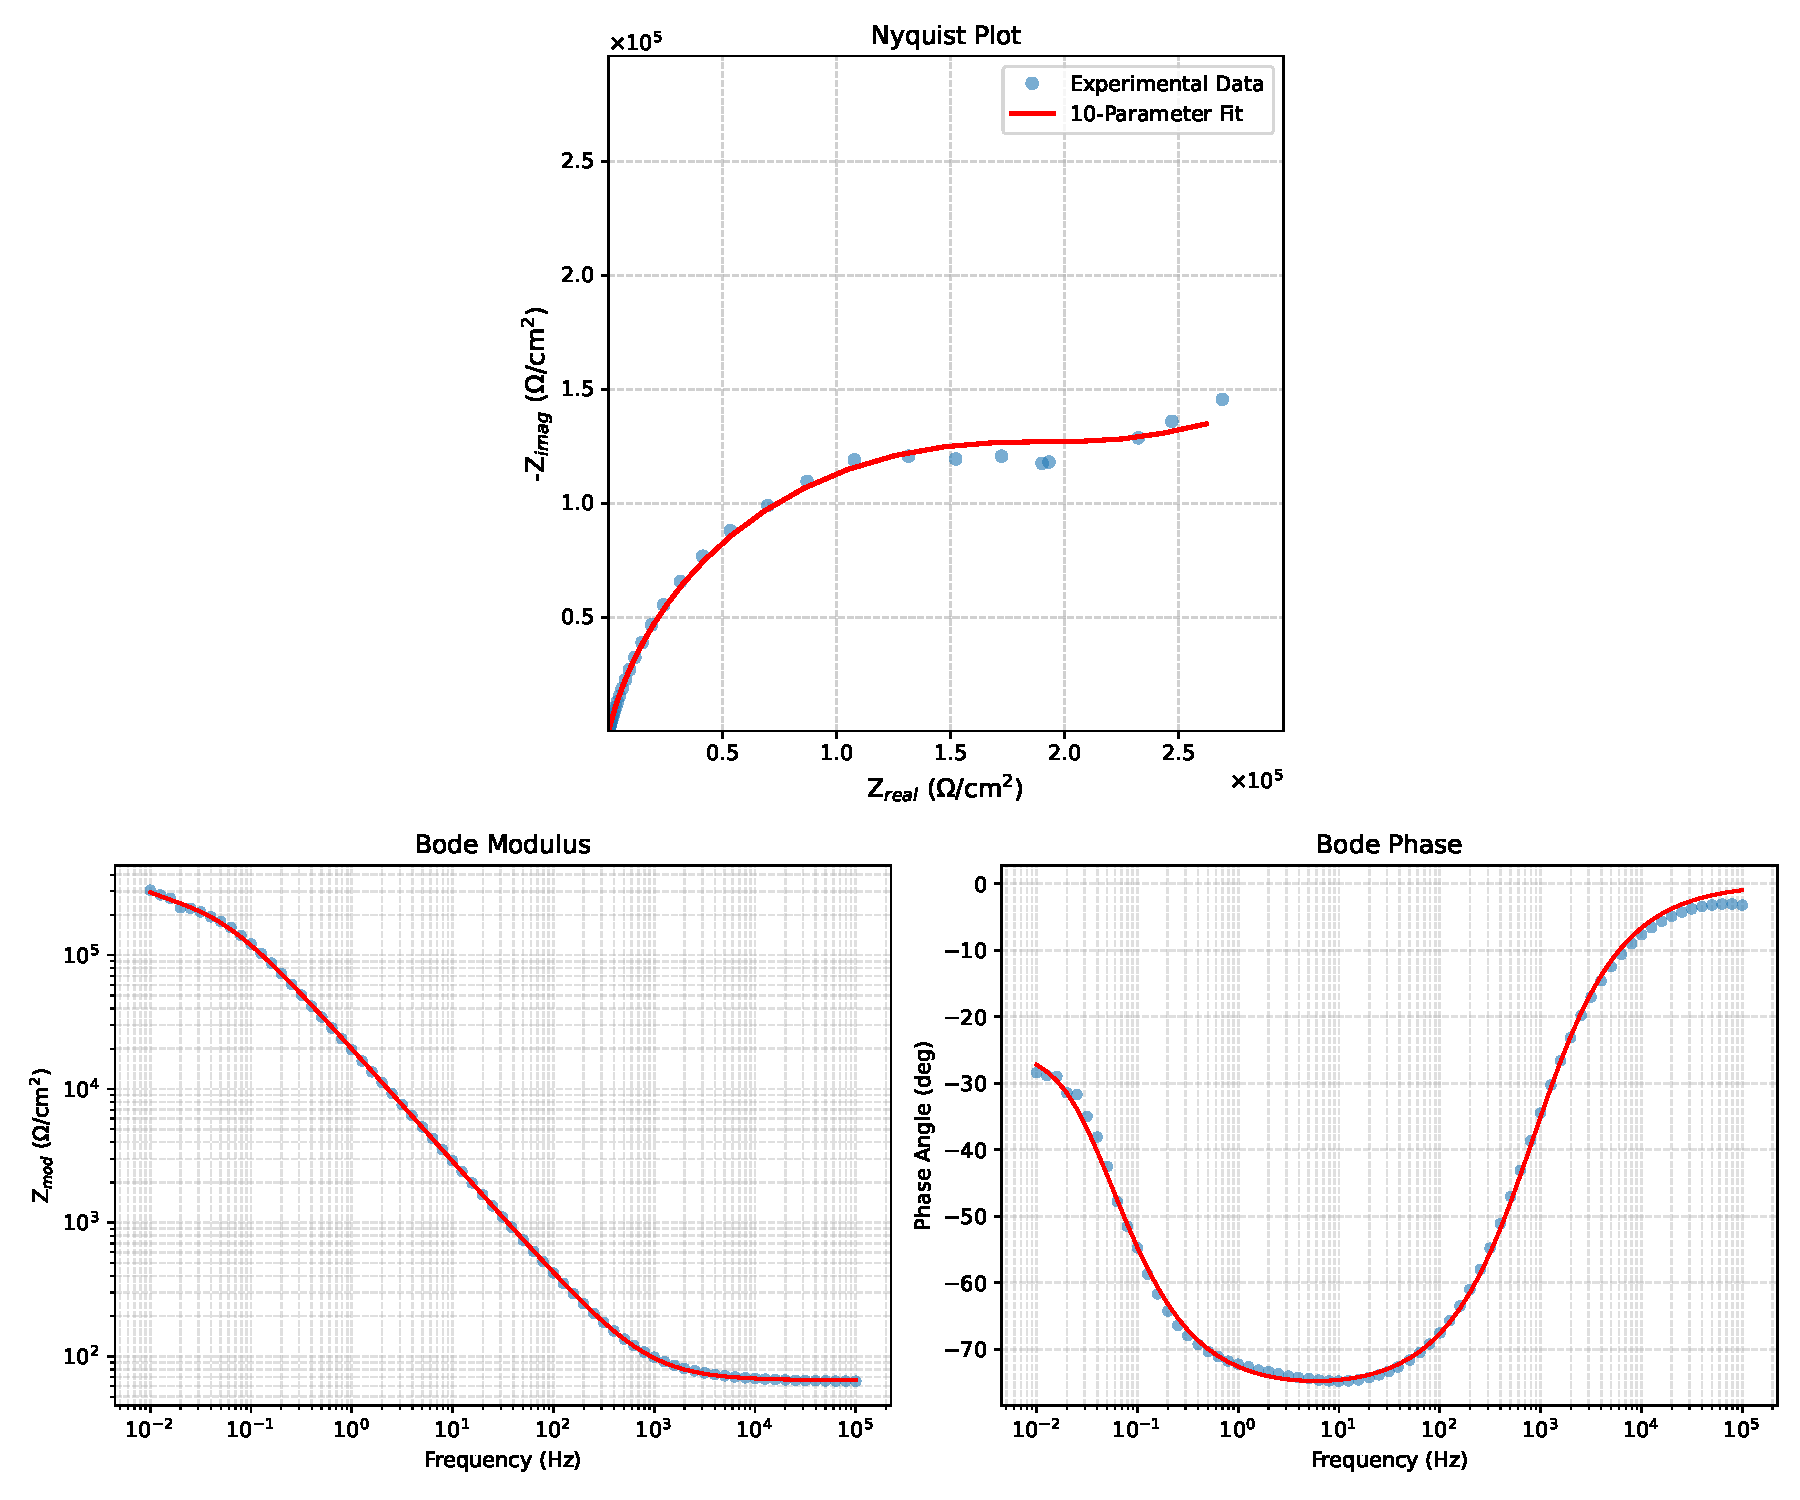
\includegraphics[width=0.7\textwidth]{plots_Cauvel_4_NaVO3_24H.pdf}
    \captionof{figure}{EIS Fit Results for Cauvel\_4\_NaVO3\_24H}
\end{center}

\newpage
\section*{Analysis Results: 48H}
\begin{center}
    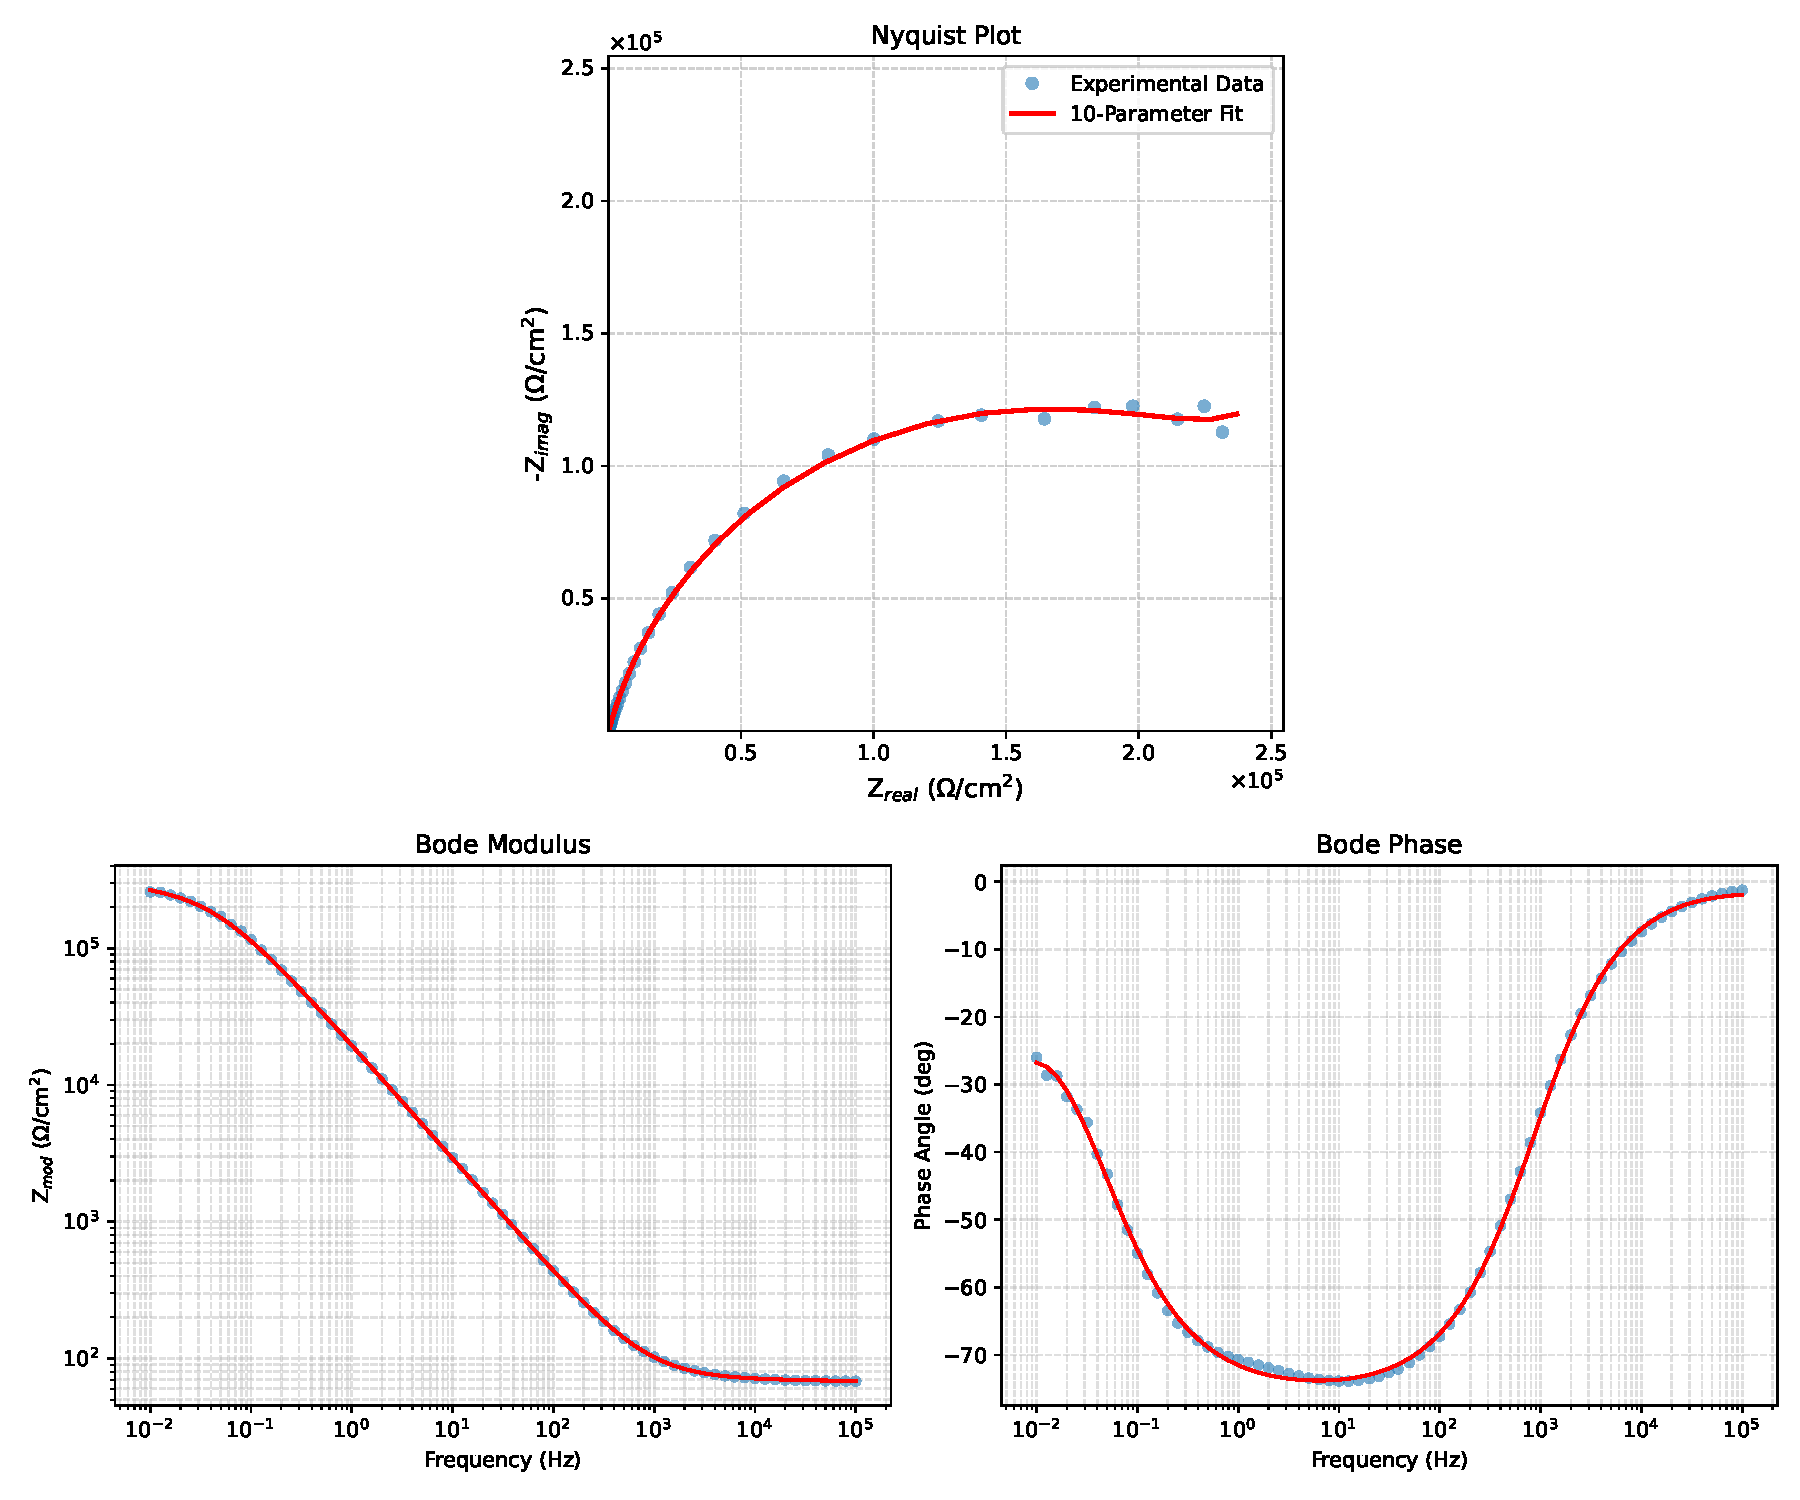
\includegraphics[width=0.7\textwidth]{plots_Cauvel_4_NaVO3_48H.pdf}
    \captionof{figure}{EIS Fit Results for Cauvel\_4\_NaVO3\_48H}
\end{center}

\newpage
\section*{Analysis Results: 72H}
\begin{center}
    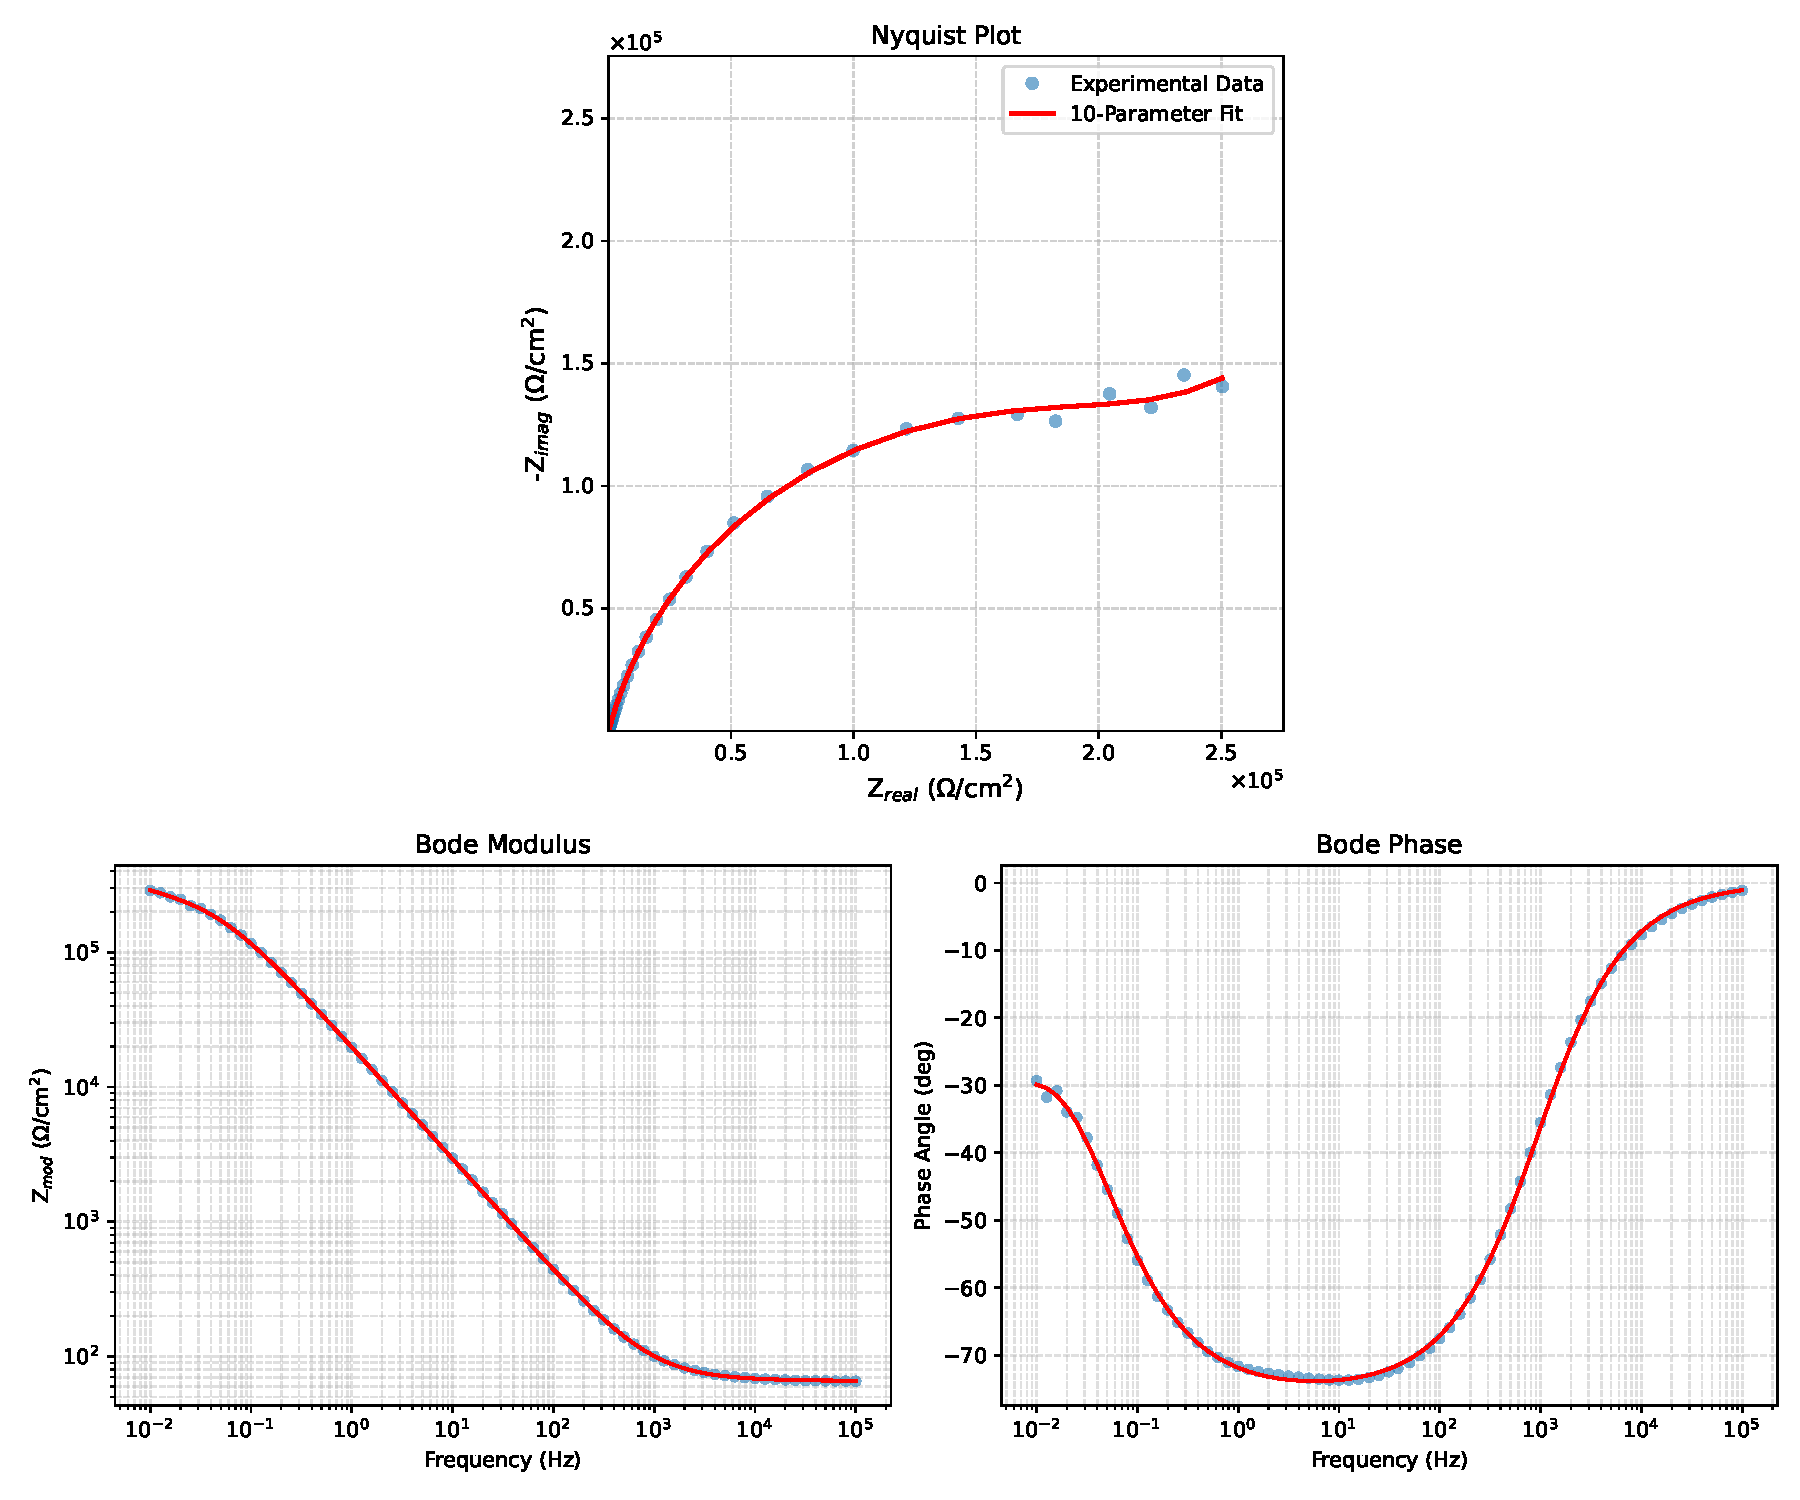
\includegraphics[width=0.7\textwidth]{plots_Cauvel_4_NaVO3_72H.pdf}
    \captionof{figure}{EIS Fit Results for Cauvel\_4\_NaVO3\_72H}
\end{center}

\newpage
\section*{Analysis Results: 168H}
\begin{center}
    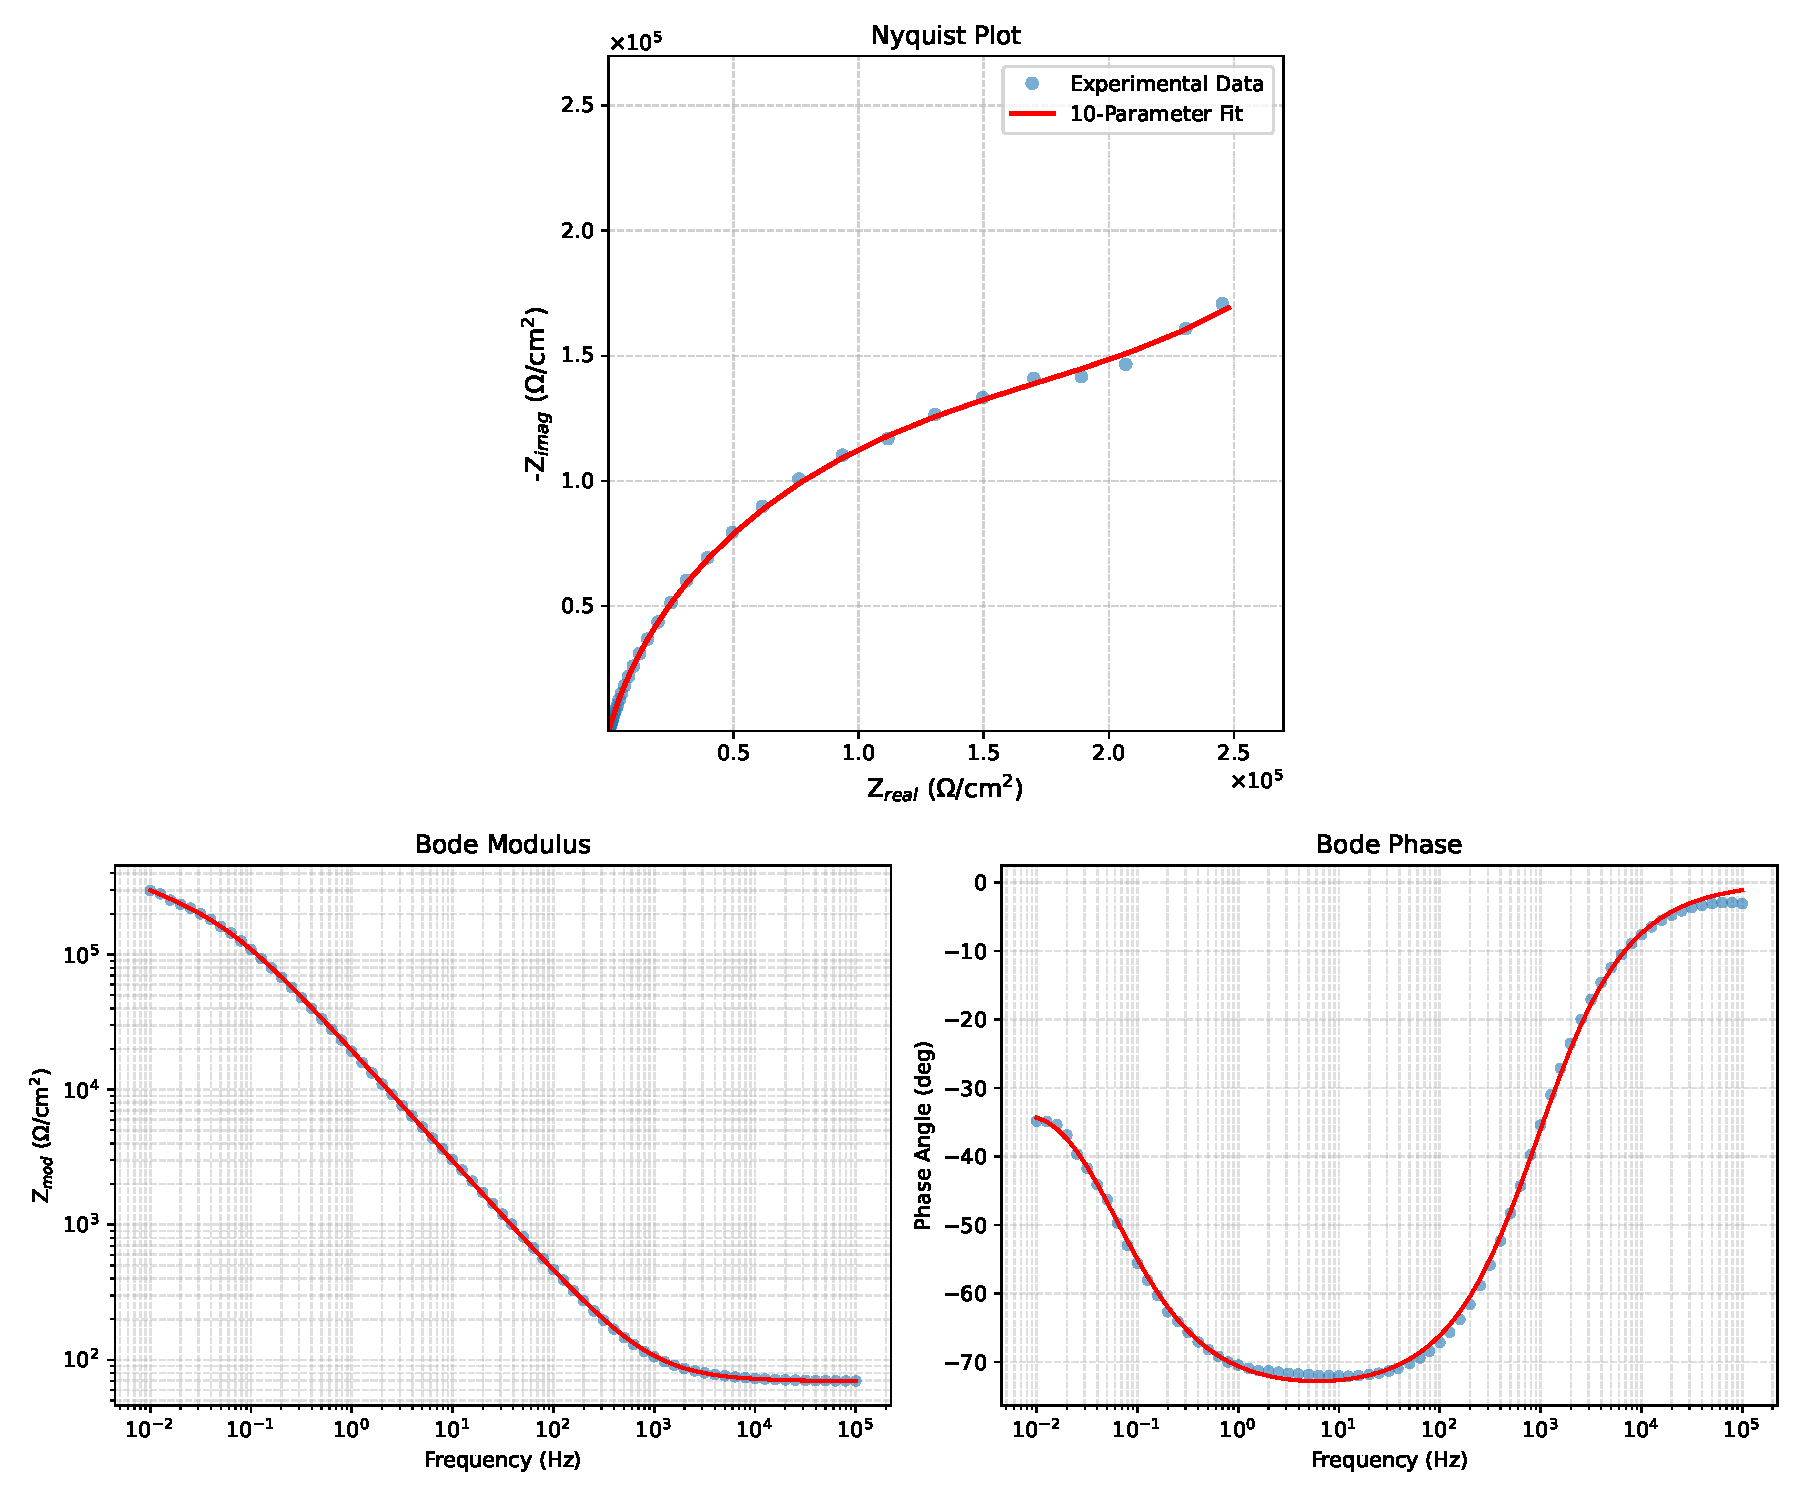
\includegraphics[width=0.7\textwidth]{plots_Cauvel_4_NaVO3_168H.pdf}
    \captionof{figure}{EIS Fit Results for Cauvel\_4\_NaVO3\_168H}
\end{center}


\end{document}
